\section{Experiments}
\label{sec:experiments}

In this section, we describe the results of our analysis of the \hoot
system with the 2008 Twitter dataset collected by Sandler and Wallach~\cite{sandler09}. This data contains 10,766,525 tweets with 255,833 hash tag references. Additionally, we show the results of experiments using our
prototype to examine the computational overhead of implementing \hoot
over all Twitter traffic.

\subsection{Cover traffic}
We first show that Twitter groups provide good possibilities for cover
traffic that \hoot can leverage to hide groups seeking plausible
deniability.

In Figure~\ref{fig:hash-dist}, we show the distribution of 
tweet volume for each hashtag in the 2008 dataset, ordered by activity
volume in a log-log scatter plot. The
distribution appears to follow a standard power law distribution, with a
few very active hashtags and many hashtags with few tweets. A large
cluster of hashtags appear only once in our dataset. 

This distribution shows us that there is a large spectrum of subscriber
anonymity set sizes that can be leveraged by \hoot. To get a high
degree of anonymity, a group organizer can choose a plain tag whose short tag
collides with a popular tag (and, thanks to the power-law
distribution, we can be confident there will always be a reasonable
distribution of plain tags, with varying popularity, to choose from).
Among other benefits, a group organizer has the ability to dial in
pretty much any amount of cover traffic for their group.

 % With such a group, the sudden influx of new
% followers will not be as suspicious. Some groups may opt
% for better plausible deniability by selecting a tag that is only
% moderately popular but serves as a believable innocuous interest for
% group members.
%gives
%you plausible deniability as there are relatively few tags dominating
%the space at a given time, and thus appear as legitimate interests. If
%there were a more even distribution of tags, then someone observing you
%following a particular tag would have less incentive to ignore suspicion
%that your activities might be objectionable to them. 

% (dwallach note: plausible deniability is discussed earlier)

\begin{figure*}[t]
\begin{minipage}[b]{0.48\linewidth}
\centering
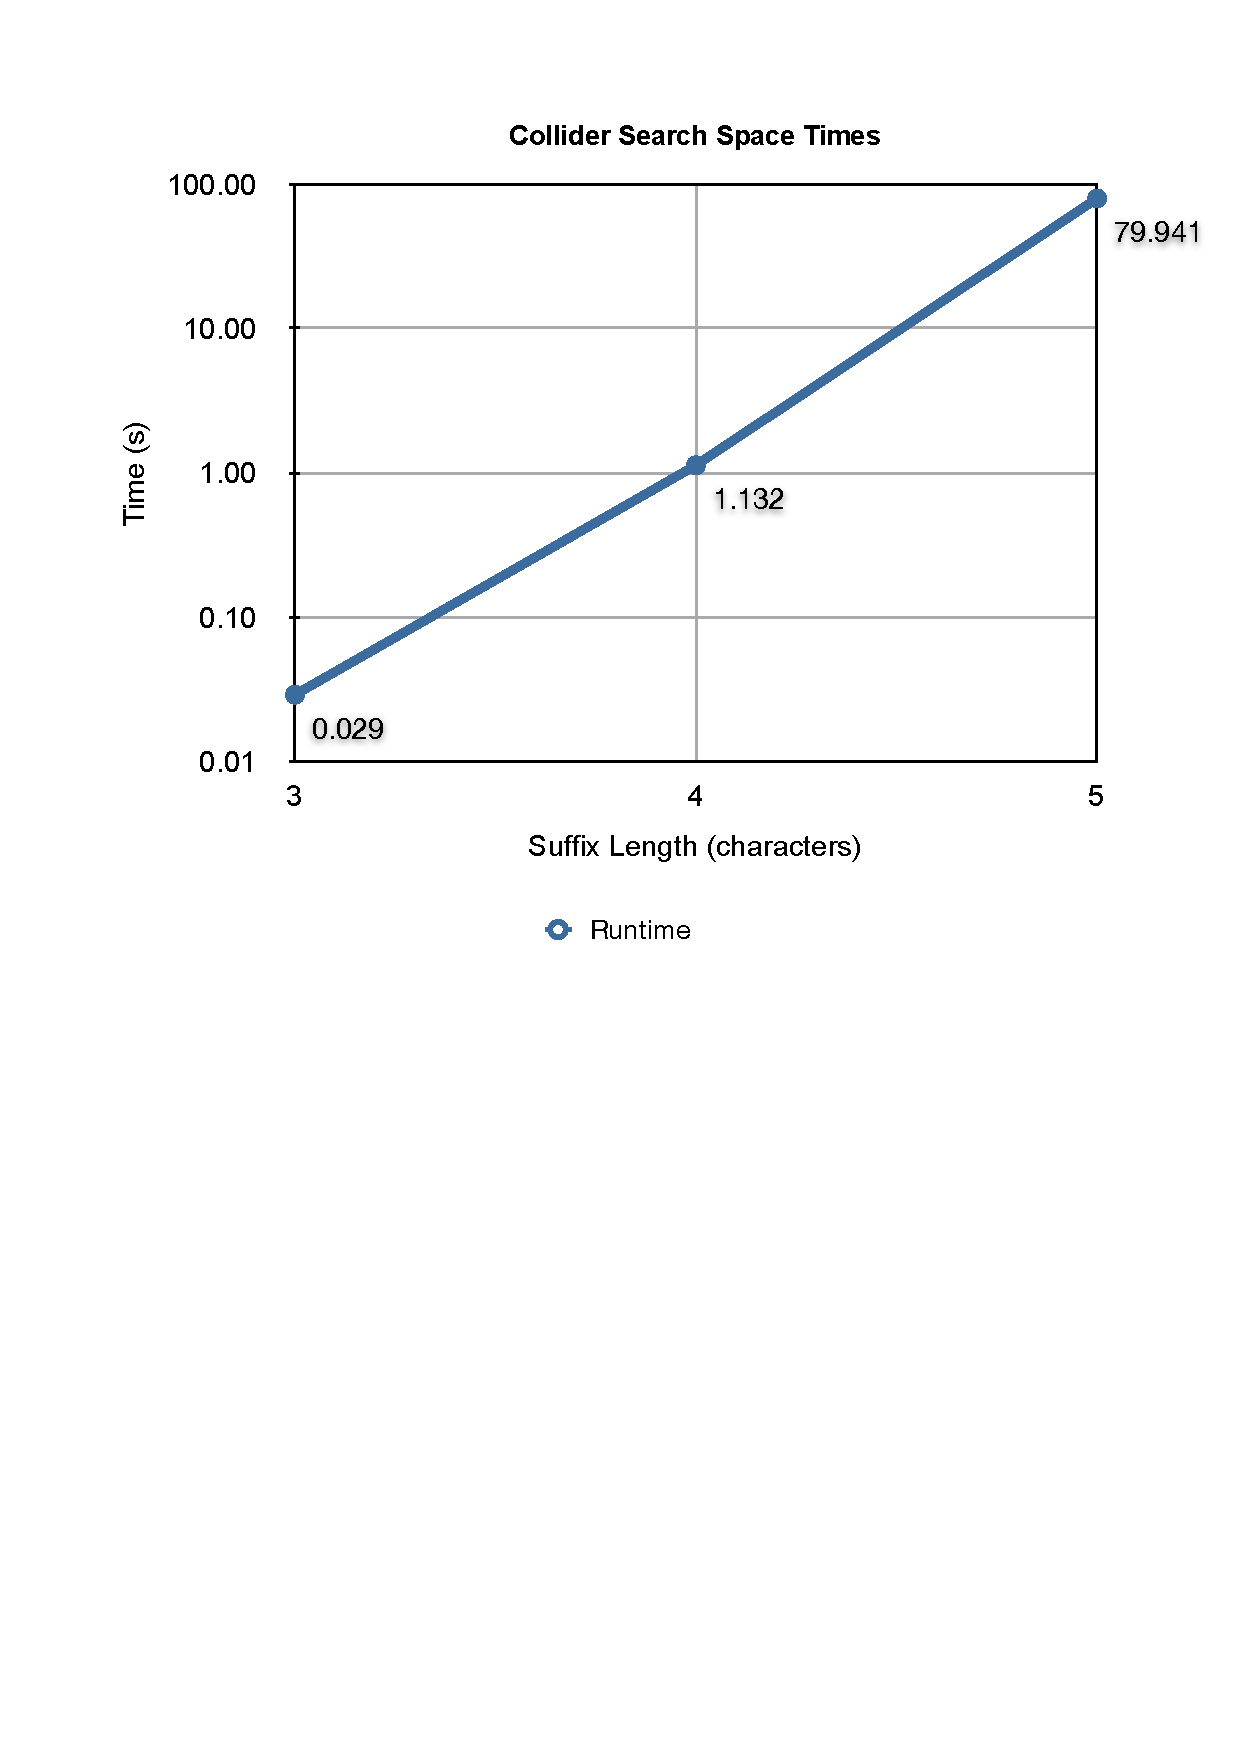
\includegraphics[scale=.5, viewport=0cm 0cm 16.6cm 13.6cm]{collider-times.pdf}
%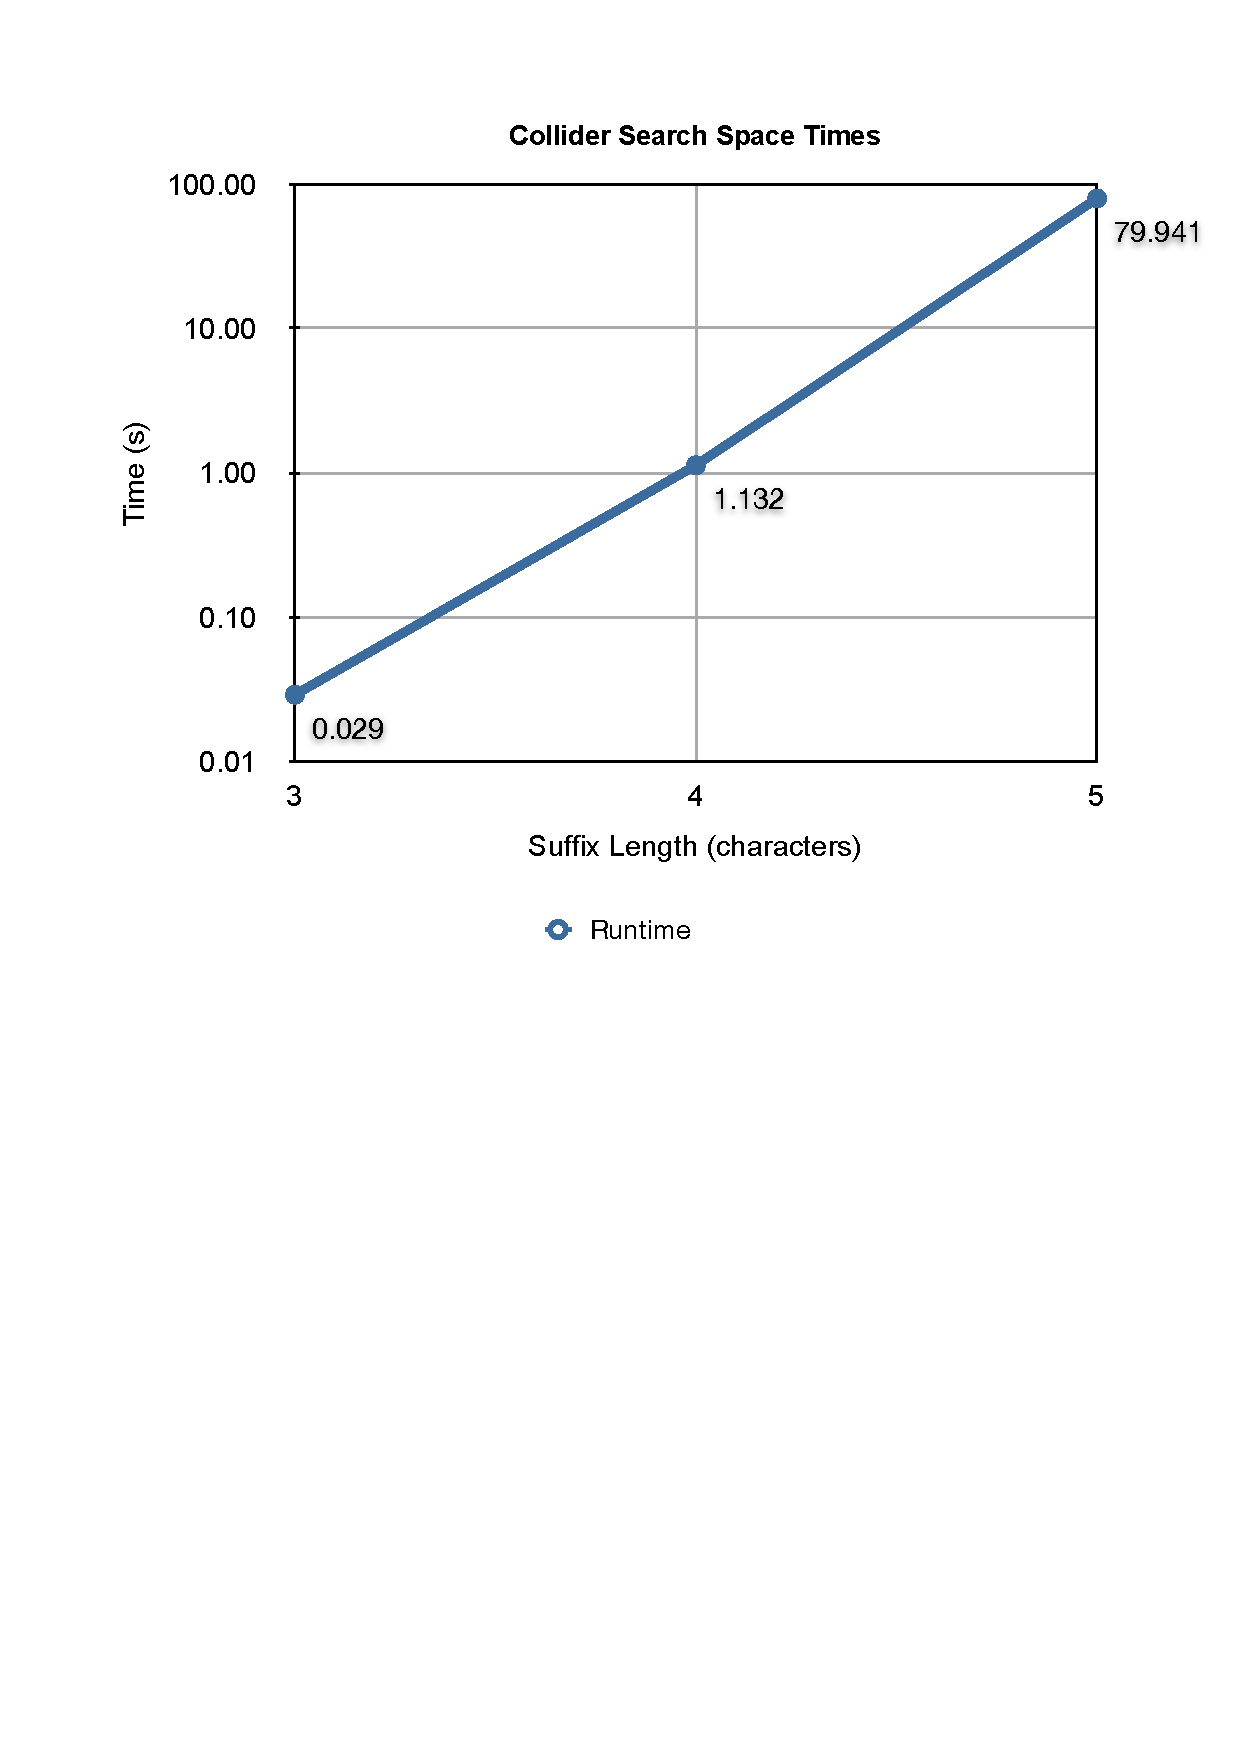
\includegraphics[scale=.5]{collider-times.pdf}
    \caption{Runtime for the collider to search for all matching tags with
  suffixes of length $L=3,4,5$ base-64 digits on a PC with dual quad-core Intel i5
  processors.}\label{fig:collider-times}
\end{minipage}
\hspace{0.5cm}
\begin{minipage}[b]{0.48\linewidth}
\centering
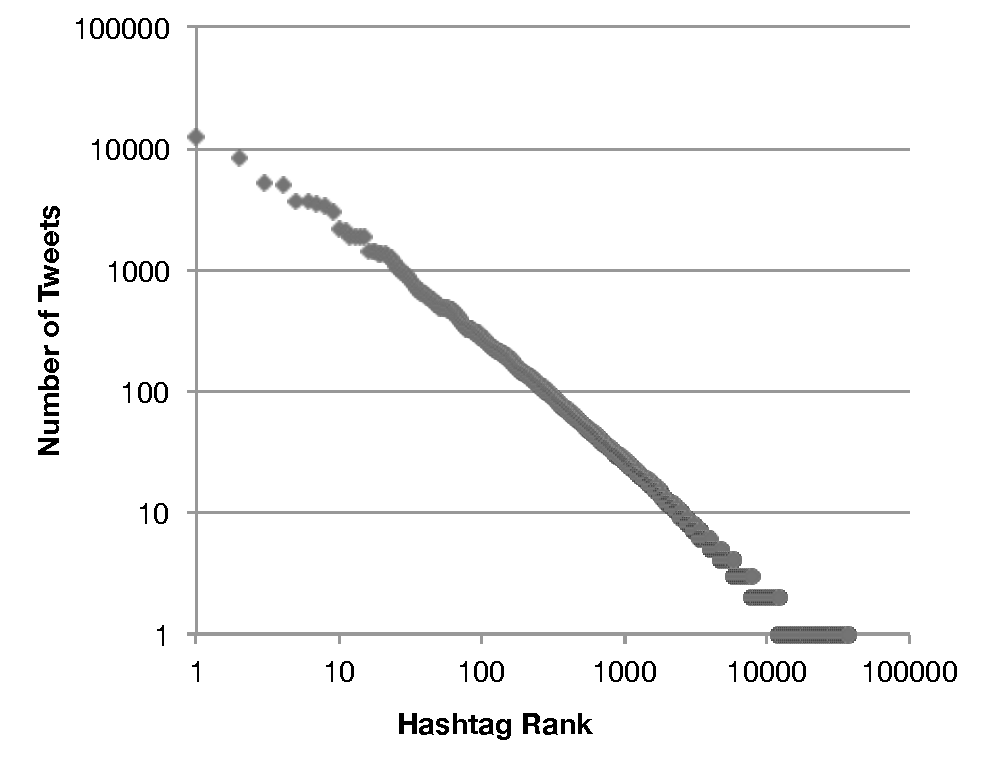
\includegraphics[scale=.5, viewport= 0cm 0cm 16.6cm 12.9cm]{hash-tag-dist.pdf}
%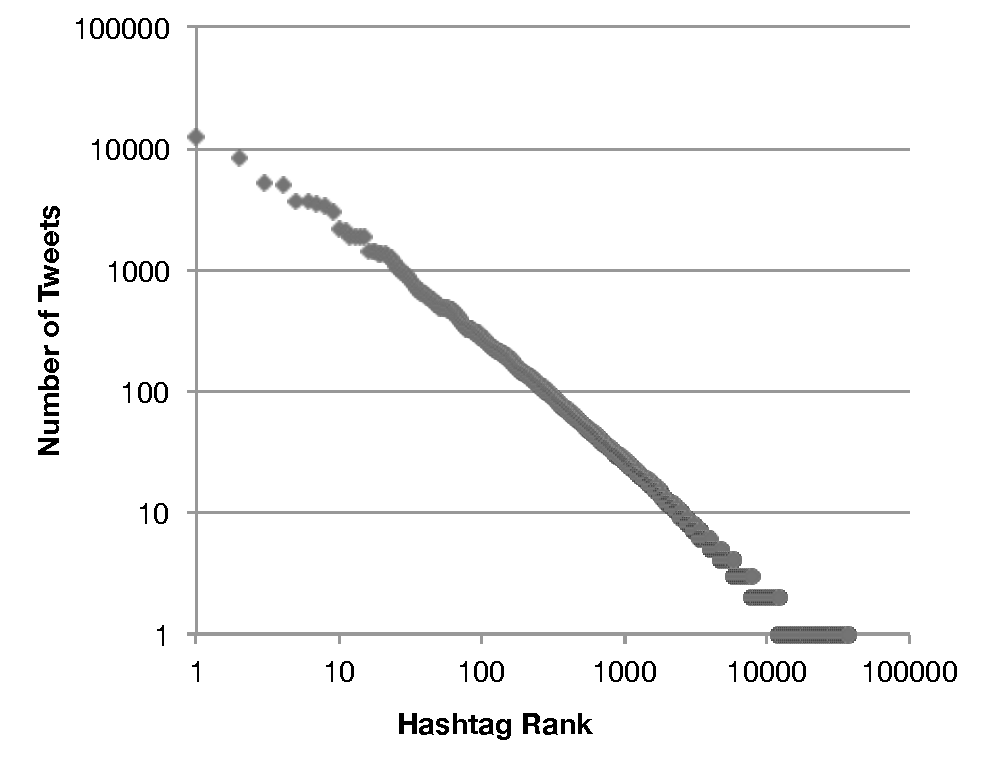
\includegraphics[scale=.5]{hash-tag-dist.pdf}
\caption{2009 Twitter hashtag activity distribution on a log-log
  scale.\vspace{0.4cm}\label{fig:hash-dist}
}
\end{minipage}
\end{figure*}

\subsection{Finding tags}
\label{sec:collider}

To explore the feasibility of finding a plain tag that collides with an
existing short tag, we built a tool called the {\em collider} in C and
OpenMP~3.0, using the open source CommonCrypto\footnote{\url{http://www.opensource.apple.com/source/CommonCrypto/}} library provided
by Apple. The collider implements the \proc{Find-Tag} algorithm
described in Figure~\ref{fig:find-tag} and is trivially parallelizable
by partitioning the search space.

\if 0
The collider takes in a short tag, \textit{T}, a prefix string,
\textit{S}, a suffix length, \textit{L}, an alphabet \textit{A}. It
finds the concatenations of \textit{S} and strings of length \textit{L}
from \textit{A*} such that the truncated hash of the resultant string
matches \textit{T}.

The collider has two modes of operation. In the default mode, the
group organizer specifies the desired number of colliding tags. The collider begins its
scan at a random point in the search space and continues scanning until
the requested number of tags are found. The second mode scans the entire
search space, and returning all matching tags for a given prefix
and suffix length.

The search space is of size $|A|^L$. If we wanted to match byte strings,
$|A| = 256$. However, since Twitter operates on characters and not
bytes, we restrict the alphabet to alphanumeric characters, yielding
$|A| = 62$. We note that the search space can be explored in parallel,
which makes the runtime of the collider executing on a system with
\textit{P} processing units $O(\frac{62^L}{P})$.

% Wow, this really is useless. We need to return the time to find one
% hit. -- dwallach
\begin{figure}
\begin{center}
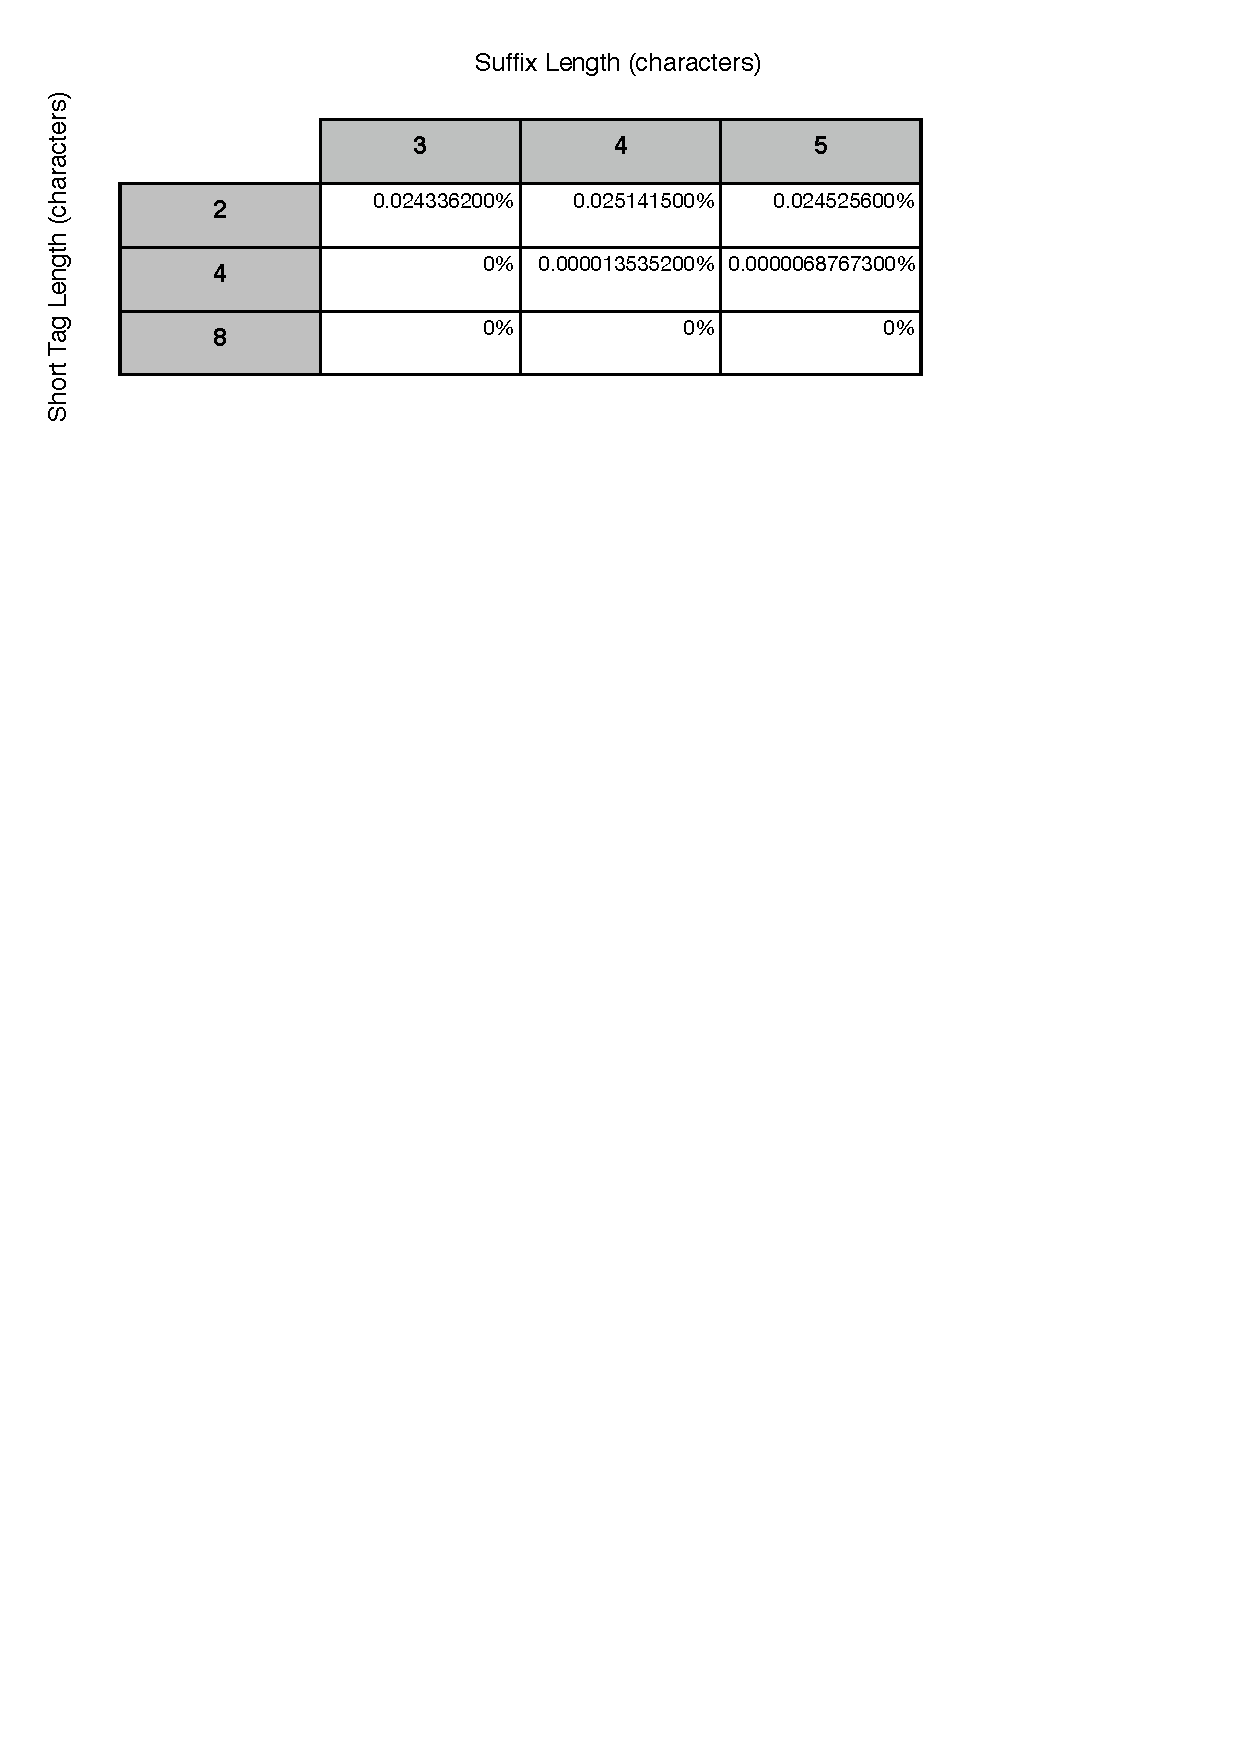
\includegraphics[scale=.5, viewport=0cm 0cm 16.5cm 7.5cm]{collider-hits.pdf}
\caption{Fraction of search space that returned hits for an entered short
  tag, with a fixed prefix and the desired suffix length (in
  Base64). We terminated the computation if no results were found in
  one day of computation.\label{fig:collider-hits}}
\end{center}
\end{figure}
\fi


As expected, the runtime
scales exponentially with the length
of the desired hash collision.
Performance is limited by the hash performance of our computer---
roughly 1.9 million ($~2^{21}$) hashes per second per core.
% dwallach-- measured on my Core 2 Duo iMac -- close enough
% for now.
Consequently, finding a collision in a short tag that's only three
Base64 digits (18 bits) takes a fraction of a second. Finding a
collision in four digits takes only a few seconds.
Even with our parallelized implementation, it is currently infeasible for a single PC to
do an exhaustive search for a suffix greater than six Base64
digits (36 bits) in less than a day.

\if 0
%Even if optimizations
%could speed up the calculation, it would likely need to take less than
%an hour to be usable for most groups. On the other hand, finding a
%collision for a short tag is proportional to its size relative to the
%search space.  \hlfixme{FiXme: What about finding one useful suffix?
%  That's the real question...}  \hlfixme{Isn't search time for a single
%  match independent of the search space of the suffix length and
%  dependent on the search space of the short tag length? Or can we not
%  assume even distribution of matching tags? Can I make that argument or
%  am I missing something?}

Another concern is the ability to find colliding tags at all. The
probability $p_{coll}$ of trying $|A|^L$ tags and finding at least one
that has the same short tag as an existing $c$-character tag is given
by:
%
\[p_{coll} = 1-\left(1-\frac{1}{|A|^c}\right)^{|A|^L}.\]
%
For an alphabet of $|A|=62$ glyphs and a short tag length of $c=2$, a
suffix of $L=3$ characters is enough to nearly guarantee at least one
collision. For a short tag length of $c=4$, a suffix of $L=5$ is
required. 
% mkw -- I can't figure out the general formula.
% The 
% \hlfixme{Numerically, on my calculator, I notice that for
%  A=62, L=c will give you prob. 0.643, and L=c+1 gives you very
%  tiny. That's not a coincidence -- find the correspondence.}

To validate this analysis with real tags, we studied the number of
collisions we could find for various values of $c$ and $L$ for a
specific prefix (``rice'') and fixed short tag values. The results,
shown in Figure~\ref{fig:collider-hits}, confirm that short tags of
length four require a suffix of length four or more to find a collision.

Thus recipient anonymity is attainable for short tags of length four or
less, and tied to this is recipient deniability. The more innocuous
traffic that is pulled, the more it seems as if you are truly following
some hot topic, rather than a more clandestine group. An observer
monitoring the tweets you download will be unable to differentiate
someone following a secret group and someone following a popular topic
because members of both groups will pulling all HooTs from each other's
groups.
\fi

%how easy it is to collide with another tag. From
%Fig. \ref{fig:collider-hits}, we find that beyond 4 characters, it was
%impossible to find collisions within easily searchable spaces (suffix
%sizes < 6).

%You can only collide with up to 4
%characters in a tag before the search space becomes such that any
%guarantee of collision is trivially small. 
%Furthermore, $62^6$ is the upper bound on the search space for what a
%single computer can reasonably calculate as a suffix to enable a
%collision. Adding one more character to the suffix sends the computation
%into the span of days on a modern computer at time of writing.
%
%However, we also show that tag collision is possible, there are certainly tunab%le degrees of anonymity thanks to the apparent power-log distribution of twitte%r tags already, and finding such a collision is feasibly done on a personal com%puter. \hl{What more to say here?}

\subsection{Overall \hoot performance}

Adoption of \hoot requires that the overhead for encryption and
decryption be minimal. For example, one path to adoption would have Twitter or
another microblogging service offer \hoot semantics over their entire
existing service. We thus consider computation overhead
in the context of encrypting {\em all} Twitter traffic as a worst case. In
March 2011, Twitter stated that the site receives 140 million tweets per
day or 1620 tweets per second on
average\footnote{\url{http://blog.twitter.com/2011/03/numbers.html}}. Twitter
also stated that the maximum number tweets per second ever was 6939. These numbers act as
rough upper bounds to the number of hoots per second the system would
need to keep up with.
% In all likelihood, the number of encrypted
% messages posted would be drastically smaller than regular messages, at
% least in the early deployment of \hoot.

\begin{table}
\caption{\hoot computation rate for encryption and
  decryption.\label{tab:hps}}
  \hlfixme{Update these values from chris's results. And make any necessary changes to the text.}
\begin{center}
    \begin{tabular}{ l  r }
	Action & Average hoots per second \\ \hline
	Encryption & 3610 \\
	Decryption & 15590 
%	Encryption & 3614.531 \\
%	Decryption & 15587.328 \\ \hline
    \end{tabular}
\end{center}
\end{table}

To study the amount of computation required to support \hoot over
Twitter, we modified our Python script to perform the encryption process 
500,000 times running on a MacBook
Air with a 1.86~GHz Intel Core~2 Duo using Base64 encoding. We 
also independently performed the decryption process 500,000 times. 
Table~\ref{tab:hps} demonstrates that the computational overhead
for \hoot cryptography is negligible for Twitter; the average
computational load can be handled by a single computer and the peak
load might require only two computers. Clearly, the issue for Twitter
or a comparable service wouldn't be cryptographic costs, it would be
bandwidth. That overhead would be entirely dependent on the selection
of the short tag on the part of the various \hoot organizers. 

On the client side, our experiments show that a modern computer can
decrypt \hoot messages significantly faster than Twitter's peak
message rate for the entirety of its traffic. (Even better, the MAC
can be validated before the message ciphertext needs to be decrypted,
providing a shortcut to skip undesired cover traffic.)  Again,
computational overhead isn't going to be the limiting factor.
Instead, the only issue will be bandwidth.

Group organizers must then take client bandwidth into account when
selecting hash collisions. An international pop music star might make
for an excellent cover story, but he might simply be too popular for
clients, particularly if the they are using cellular phone networks
that haven't been brought up to the latest multi-megabit speeds.
This is the one place where the short size of Twitter
messages actually works in our favor. A modest data pipe of 128
kbits/sec can transmit roughly 114 tweets per second. This is well
within the regular bounds of most any short tag selected by the group
organizers.

Assuming the entire peak load 7000-or-so tweets per second ends up
split uniformly across short tags with three base-64 digits (i.e., 18
bit short tags), the average number of tweets per second per short tag
is only 0.02 (i.e., only 1.6 \hoot messages per minute). That's well
within any realistic bandwidth constraint.


\if 0


The decryption rate is important to clients, since clients will need to
search through hoots with colliding hashtags and decrypt the session
keys for each one to see if it decrypts correctly. Note that, with a
simple fixed constant string prepended to the keys, the client can
quickly verify whether the message was encrypted using $k_{tag}$ or if
another group's key was used. Since our process can decrypt Hoots almost
five times faster than it encrypts them, even clients with limited
computing power can keep up with the entire Twitter feed. In practice,
clients would only need to decrypt hoots that share the same short tag,
which should be a small fraction of this cost even for very active
groups.

%A client may not trust Twitter to do the decryption since that involves
%sharing the plain tag with Twitter, so a client would decrypt the
%message on their machine. Almost every client will not have a datacenter
%of computers for decryption, but 
%adopted with little engineering effort.

%\hl{Should experiments have a wrap up paragraph?}

%\hlfxnote{mkw -- I don't think so. We'll cover more ground in the discussion.}

\fi
